\documentclass[a4paper,10pt]{article}
\usepackage[left=0.6in,right=0.6in,top=0.6in,bottom=0.6in]{geometry}
\usepackage{graphicx}
\usepackage{tabularx}
\usepackage{enumitem}
\usepackage{hyperref}
\usepackage{titlesec}
\usepackage{xcolor}

\pagestyle{empty}

% Custom section formatting to match reference exactly
\newcommand{\cvsection}[1]{
    \vspace{1ex}
    \hrule
    \vspace{0.5ex}
    \begin{center}
        \textbf{\MakeUppercase{#1}}
    \end{center}
    \vspace{-1.5ex}
    \hrule
    \vspace{1ex}
}

\begin{document}

% Header
\noindent
\begin{minipage}[c]{0.15\textwidth}
    % Uncomment and replace with actual logo file path if available
    % \includegraphics[height=2cm]{logo.png} 
\end{minipage}%
\begin{minipage}[c]{0.7\textwidth}
    \centering
    {\Huge \textbf{GANESH MAHATA}}\\[0.2em]
\end{minipage}%
\begin{minipage}[c]{0.15\textwidth}
    \raggedleft
    % Uncomment and replace with actual profile photo file path
    % 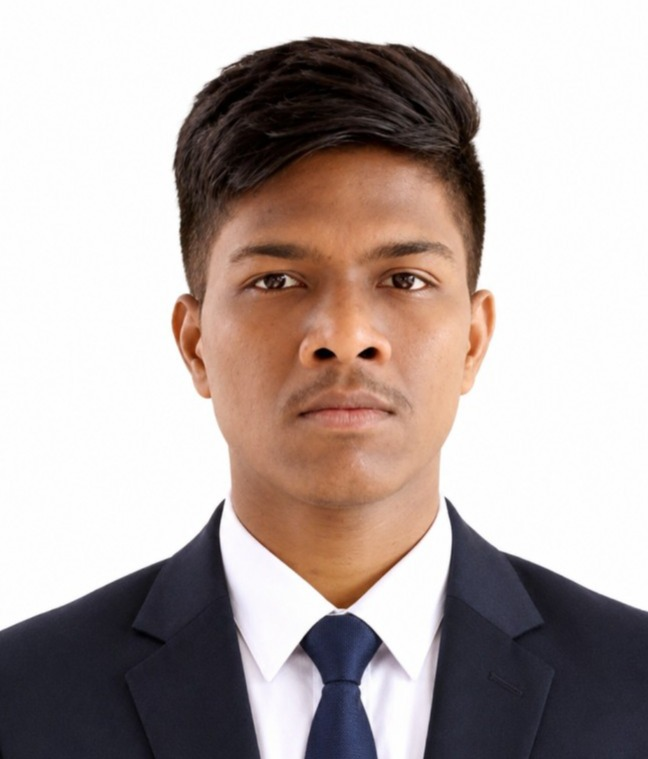
\includegraphics[height=2.5cm]{assets/images/profile.jpeg}
\end{minipage}

\vspace{0.5em}

\cvsection{Academic Details}
\vspace{-1ex}
\begin{center}
\renewcommand{\arraystretch}{1.2}
\begin{tabular*}{\textwidth}{@{\extracolsep{\fill}} l c l c}
\hline
\textbf{Year} & \textbf{Degree / Board} & \textbf{Institute} & \textbf{GPA / Marks(\%)} \\
\hline
2022 - Present & B.Tech in Biotechnology & Indian Institute of Technology Delhi & Ongoing \\
Until 2022 & Class XII (Science) & Jawahar Navodaya Vidyalaya (JNV), Bankura & - \\
\hline
\end{tabular*}
\end{center}

\cvsection{Scholastic Achievements \& Certifications}
\begin{itemize}[leftmargin=1.5em, noitemsep, topsep=0pt]
    \item \textbf{Python Programming Fundamentals} -- Online
    \item \textbf{HTML, CSS \& JavaScript - Full Course} -- Online
    \item \textbf{Git \& GitHub - Version Control} -- Online
    \item \textbf{Arduino \& ESP32 Development} -- Self-study
\end{itemize}

\cvsection{Projects}
\begin{itemize}[leftmargin=1.5em, noitemsep, itemsep=0.8ex, topsep=0pt]
    \item \textbf{ESP32 IoT Monitoring System} \hfill [2024] \\
    - Real-time sensor monitoring with ESP32, OLED display, and Google Sheets cloud logging.\\
    - Tech Stack: ESP32, C++, Wi-Fi
    
    \item \textbf{Grafana IoT Dashboard} \hfill [2024] \\
    - Live data visualization using Grafana connected to IoT sensor streams.\\
    - Tech Stack: Grafana, Python, ESP32
    
    \item \textbf{IIT Department Website} \hfill [2023] \\
    - Fully responsive academic website with structured content and clean UI.\\
    - Tech Stack: HTML5, CSS3, JavaScript
    
    \item \textbf{RFID Access Control System} \hfill [2023] \\
    - RFID-based door access control with Arduino and event logging.\\
    - Tech Stack: Arduino, RFID, C++
\end{itemize}

\cvsection{Technical Skills}
\begin{itemize}[leftmargin=1.5em, noitemsep, topsep=0pt]
    \item \textbf{Programming Languages:} Python, C, C++, JavaScript, HTML5, CSS3, SQL
    \item \textbf{Embedded / IoT:} Arduino UNO, ESP32, ESP8266, NodeMCU, RFID, OLED
    \item \textbf{Web Development:} HTML5, CSS3, JavaScript, Responsive, GitHub Pages
    \item \textbf{Tools \& Databases:} Git / GitHub, VS Code, Grafana, Firebase, Supabase
\end{itemize}

\cvsection{Research Interests \& Currently Learning}
\begin{itemize}[leftmargin=1.5em, noitemsep, topsep=0pt]
    \item \textbf{Research Interests:} Smart Healthcare, Biomedical Devices, AI for Biotechnology, Embedded Medical Devices, IoT-Based Monitoring, Sustainable Technologies
    \item \textbf{Currently Learning:} Advanced JavaScript, Git \& GitHub, ESP32 Development, Grafana Dashboards, Database Integration, Cloud Services
\end{itemize}

\vfill
\noindent\textit{Disclaimer: All the information on this page is entered by student.} \hfill \textbf{Page 1}

\end{document}
